% ============================================================
% Cataract Classification using Explainable AI - Project Report
% ============================================================
\documentclass[12pt, a4paper]{article}

% ── Packages ──
\usepackage[utf8]{inputenc}
\usepackage[T1]{fontenc}
\usepackage{geometry}
\geometry{margin=2.5cm}
\usepackage{graphicx}
\usepackage{booktabs}
\usepackage{hyperref}
\usepackage{amsmath}
\usepackage{enumitem}
\usepackage{float}
\usepackage{caption}
\usepackage{subcaption}
\usepackage{listings}
\usepackage{xcolor}
\usepackage{titlesec}
\usepackage{setspace}
\onehalfspacing

\hypersetup{
    colorlinks=true,
    linkcolor=blue,
    citecolor=blue,
    urlcolor=blue
}

% Code listing style
\lstset{
    basicstyle=\ttfamily\small,
    breaklines=true,
    frame=single,
    backgroundcolor=\color{gray!10},
    keywordstyle=\color{blue},
    commentstyle=\color{green!60!black},
    stringstyle=\color{red!70!black},
    language=Python
}

% ── Title Page ──
\begin{document}

\begin{titlepage}
\centering
\vspace*{2cm}

{\LARGE\bfseries Cataract Classification from Retinal Fundus Images\\using Explainable AI\par}

\vspace{1.5cm}

{\large A Project Report\par}
\vspace{0.5cm}
{\large Submitted in partial fulfillment of the requirements for the degree of\par}
\vspace{0.5cm}
{\large\bfseries Bachelor of Technology\par}
\vspace{0.3cm}
{\large in\par}
\vspace{0.3cm}
% ── EDIT THIS: Your department name ──
{\large\bfseries Computer Science and Engineering\par}

\vspace{2cm}

{\large Submitted by:\par}
\vspace{0.3cm}
% ── EDIT THIS: Your name and roll number ──
{\large\bfseries Your Name (Roll No: XXXXXXXXXX)\par}

\vspace{1.5cm}

{\large Under the guidance of:\par}
\vspace{0.3cm}
% ── EDIT THIS: Guide name ──
{\large\bfseries Prof. Guide Name\par}

\vspace{2cm}

% ── EDIT THIS: College name ──
{\large Department of Computer Science and Engineering\\
Your College Name\\
City, Year\par}

\end{titlepage}

% ── Table of Contents ──
\newpage
\tableofcontents
\newpage

% ============================================================
% 1. ABSTRACT
% ============================================================
\section{Abstract}

Cataract is a leading cause of avoidable blindness, characterized by opacification of the eye's crystalline lens. Early detection through automated screening can help reduce the burden on ophthalmologists. This project presents a deep learning based system for binary classification of retinal fundus images as cataract or normal, with Grad-CAM heatmaps providing visual explanations of model decisions.

The system uses the ODIR-5K (Ocular Disease Intelligent Recognition) dataset, containing 7,000 fundus images from 3,500 patients. After filtering for eyes with exact diagnostic keywords ``cataract'' or ``normal fundus'', 3,078 images (262 cataract, 2,816 normal) were retained. Two transfer learning models—ResNet50 and EfficientNet-B0—were fine-tuned with ImageNet pretrained weights, weighted binary cross-entropy loss to handle class imbalance, and patient-level data splitting to prevent data leakage.

On the held-out test set (448 images), ResNet50 achieved 96.88\% accuracy with an ROC-AUC of 0.9676, while EfficientNet-B0 achieved 95.31\% accuracy with an ROC-AUC of 0.9848. ResNet50 was selected as the deployed model based on the highest validation ROC-AUC (0.9953). Grad-CAM heatmaps demonstrate that the model focuses on clinically relevant regions of the fundus image. A Streamlit web application allows interactive classification of uploaded fundus images with real-time Grad-CAM overlays.

\textbf{Keywords:} cataract detection, fundus photography, ODIR, transfer learning, Grad-CAM, explainable AI

% ============================================================
% 2. INTRODUCTION
% ============================================================
\section{Introduction}

\subsection{Background}
Cataract is an opacification of the crystalline lens of the eye and is a leading cause of avoidable vision impairment worldwide. According to the World Health Organization, cataracts account for approximately 51\% of world blindness. Early detection and timely surgical intervention can restore vision, but manual screening by ophthalmologists is time-consuming and resource-intensive, especially in rural areas.

A fundus camera photographs the retina through the lens, so cataract can appear as haze, lower contrast, or uneven illumination rather than as a distinct focal lesion. This makes it possible for deep learning models to learn patterns from fundus images that distinguish cataract-affected eyes from normal ones.

\subsection{Problem Statement}
The challenge is to develop an automated system that can:
\begin{enumerate}
    \item Accurately classify retinal fundus images as cataract or normal.
    \item Provide visual explanations of why the model made a particular prediction, increasing trust and clinical interpretability.
    \item Handle the significant class imbalance inherent in medical datasets (only 8.5\% of images are cataract).
\end{enumerate}

\subsection{Objectives}
\begin{itemize}
    \item Build a reproducible eye-level dataset of cataract versus normal from ODIR-5K.
    \item Ensure patient-level splitting so both eyes of a patient remain in the same data split.
    \item Fine-tune ImageNet pretrained ResNet50 and EfficientNet-B0 for binary cataract classification.
    \item Compare model performance using accuracy, precision, recall, F1-score, ROC-AUC, and PR-AUC.
    \item Apply Grad-CAM to visualize which image regions influenced the model's decision.
    \item Build a Streamlit demo application for interactive classification with explanations.
\end{itemize}

% ============================================================
% 3. LITERATURE REVIEW
% ============================================================
\section{Literature Review}

Cataract detection from fundus images has been studied using various approaches:

\begin{itemize}
    \item \textbf{Traditional methods:} Earlier approaches used handcrafted features (edge detection, texture analysis) with classifiers like SVM and Random Forest, achieving moderate accuracy \cite{yang2016}.
    \item \textbf{CNN-based methods:} Convolutional neural networks significantly improved detection accuracy. Studies using VGG, ResNet, and Inception architectures on ODIR and similar datasets reported accuracies above 90\% \cite{ali2022}.
    \item \textbf{Transfer learning:} Pretrained ImageNet models fine-tuned on medical imaging tasks have shown strong performance even with limited training data \cite{raghu2019}.
    \item \textbf{EfficientNet:} Tan and Le proposed EfficientNet, which achieves better accuracy with fewer parameters through compound scaling \cite{tan2019}.
    \item \textbf{Explainable AI:} Selvaraju et al. proposed Grad-CAM, which produces visual explanations by using the gradients of the target class flowing into the final convolutional layer \cite{selvaraju2017}.
    \item \textbf{ODIR dataset:} Li et al. released the ODIR-5K dataset for the 2019 Ocular Disease Intelligent Recognition challenge, containing multi-label eye disease annotations \cite{li2021}.
\end{itemize}

% ============================================================
% 4. SOFTWARE AND HARDWARE REQUIREMENTS
% ============================================================
\section{Software and Hardware Requirements}

\subsection{Software Requirements}
\begin{table}[H]
\centering
\begin{tabular}{@{}ll@{}}
\toprule
\textbf{Component} & \textbf{Specification} \\
\midrule
Operating System & Windows 11 \\
Programming Language & Python 3.12 \\
Deep Learning Framework & PyTorch 2.6.0 + CUDA 12.4 \\
Computer Vision & torchvision 0.21.0, OpenCV 4.10 \\
Data Processing & NumPy 1.26, Pandas 2.2 \\
Machine Learning & scikit-learn 1.5 \\
Visualization & Matplotlib 3.8, Seaborn 0.13 \\
Explainable AI & pytorch-grad-cam 1.5 \\
Web Application & Streamlit 1.67 \\
\bottomrule
\end{tabular}
\caption{Software requirements}
\end{table}

\subsection{Hardware Requirements}
\begin{table}[H]
\centering
\begin{tabular}{@{}ll@{}}
\toprule
\textbf{Component} & \textbf{Specification} \\
\midrule
Processor & Intel Core (or AMD equivalent) \\
RAM & 8 GB minimum (16 GB recommended) \\
GPU & NVIDIA GeForce RTX 2050 (4 GB VRAM) \\
Storage & 5 GB free disk space \\
CUDA Version & 12.4 \\
\bottomrule
\end{tabular}
\caption{Hardware requirements}
\end{table}

% ============================================================
% 5. DATASET
% ============================================================
\section{Dataset}

\subsection{ODIR-5K Dataset}
The Ocular Disease Intelligent Recognition (ODIR-5K) dataset was released for the ODIR 2019 challenge. It contains 7,000 color fundus photographs from 3,500 patients, with left-eye and right-eye images and diagnostic keywords for each eye. The dataset includes labels for eight conditions: normal, diabetes, glaucoma, cataract, age-related macular degeneration, hypertension, myopia, and other abnormalities.

\subsection{Label Construction}
Each patient record was split into two eye-level records. The cataract label (1) was assigned to eyes whose diagnostic keyword was exactly ``cataract''. The normal label (0) was assigned to eyes with keyword exactly ``normal fundus''. Eyes with mixed diseases, other conditions, or ambiguous keywords were excluded. The patient-level disease columns were not used as the eye-level label to avoid mislabeling.

This filtering yielded \textbf{3,078 images} from 1,951 patients: 262 cataract (8.5\%) and 2,816 normal (91.5\%).

\subsection{Data Splitting}
Patients were shuffled with seed 42 and split 70\%/15\%/15\% at the patient level, ensuring both eyes of a patient stay in the same split to prevent data leakage.

\begin{table}[H]
\centering
\begin{tabular}{@{}lcccc@{}}
\toprule
\textbf{Split} & \textbf{Patients} & \textbf{Images} & \textbf{Cataract} & \textbf{Normal} \\
\midrule
Train & 1,365 & 2,175 & 186 & 1,989 \\
Validation & 293 & 455 & 31 & 424 \\
Test & 293 & 448 & 45 & 403 \\
\midrule
\textbf{Total} & \textbf{1,951} & \textbf{3,078} & \textbf{262} & \textbf{2,816} \\
\bottomrule
\end{tabular}
\caption{Patient-disjoint train/validation/test splits}
\end{table}

% ── FIGURE: Class Distribution ──
% Copy outputs/plots/class_distribution.png → report/figures/
\begin{figure}[H]
\centering
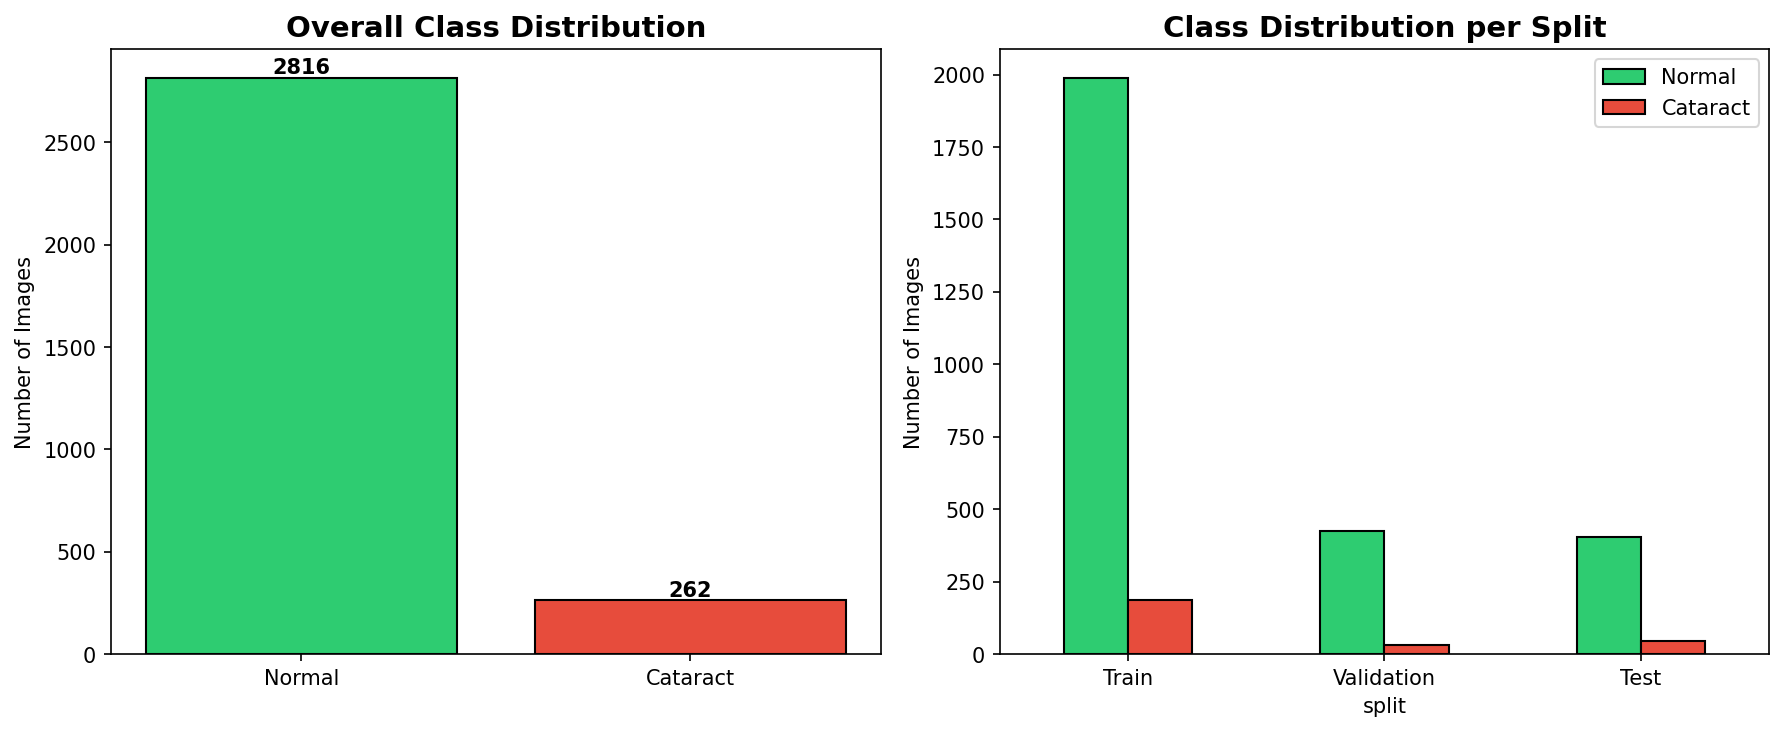
\includegraphics[width=0.95\textwidth]{figures/class_distribution.png}
\caption{Class distribution in the overall dataset and per split.}
\label{fig:class_dist}
\end{figure}

% ── FIGURE: Sample Images ──
\begin{figure}[H]
\centering
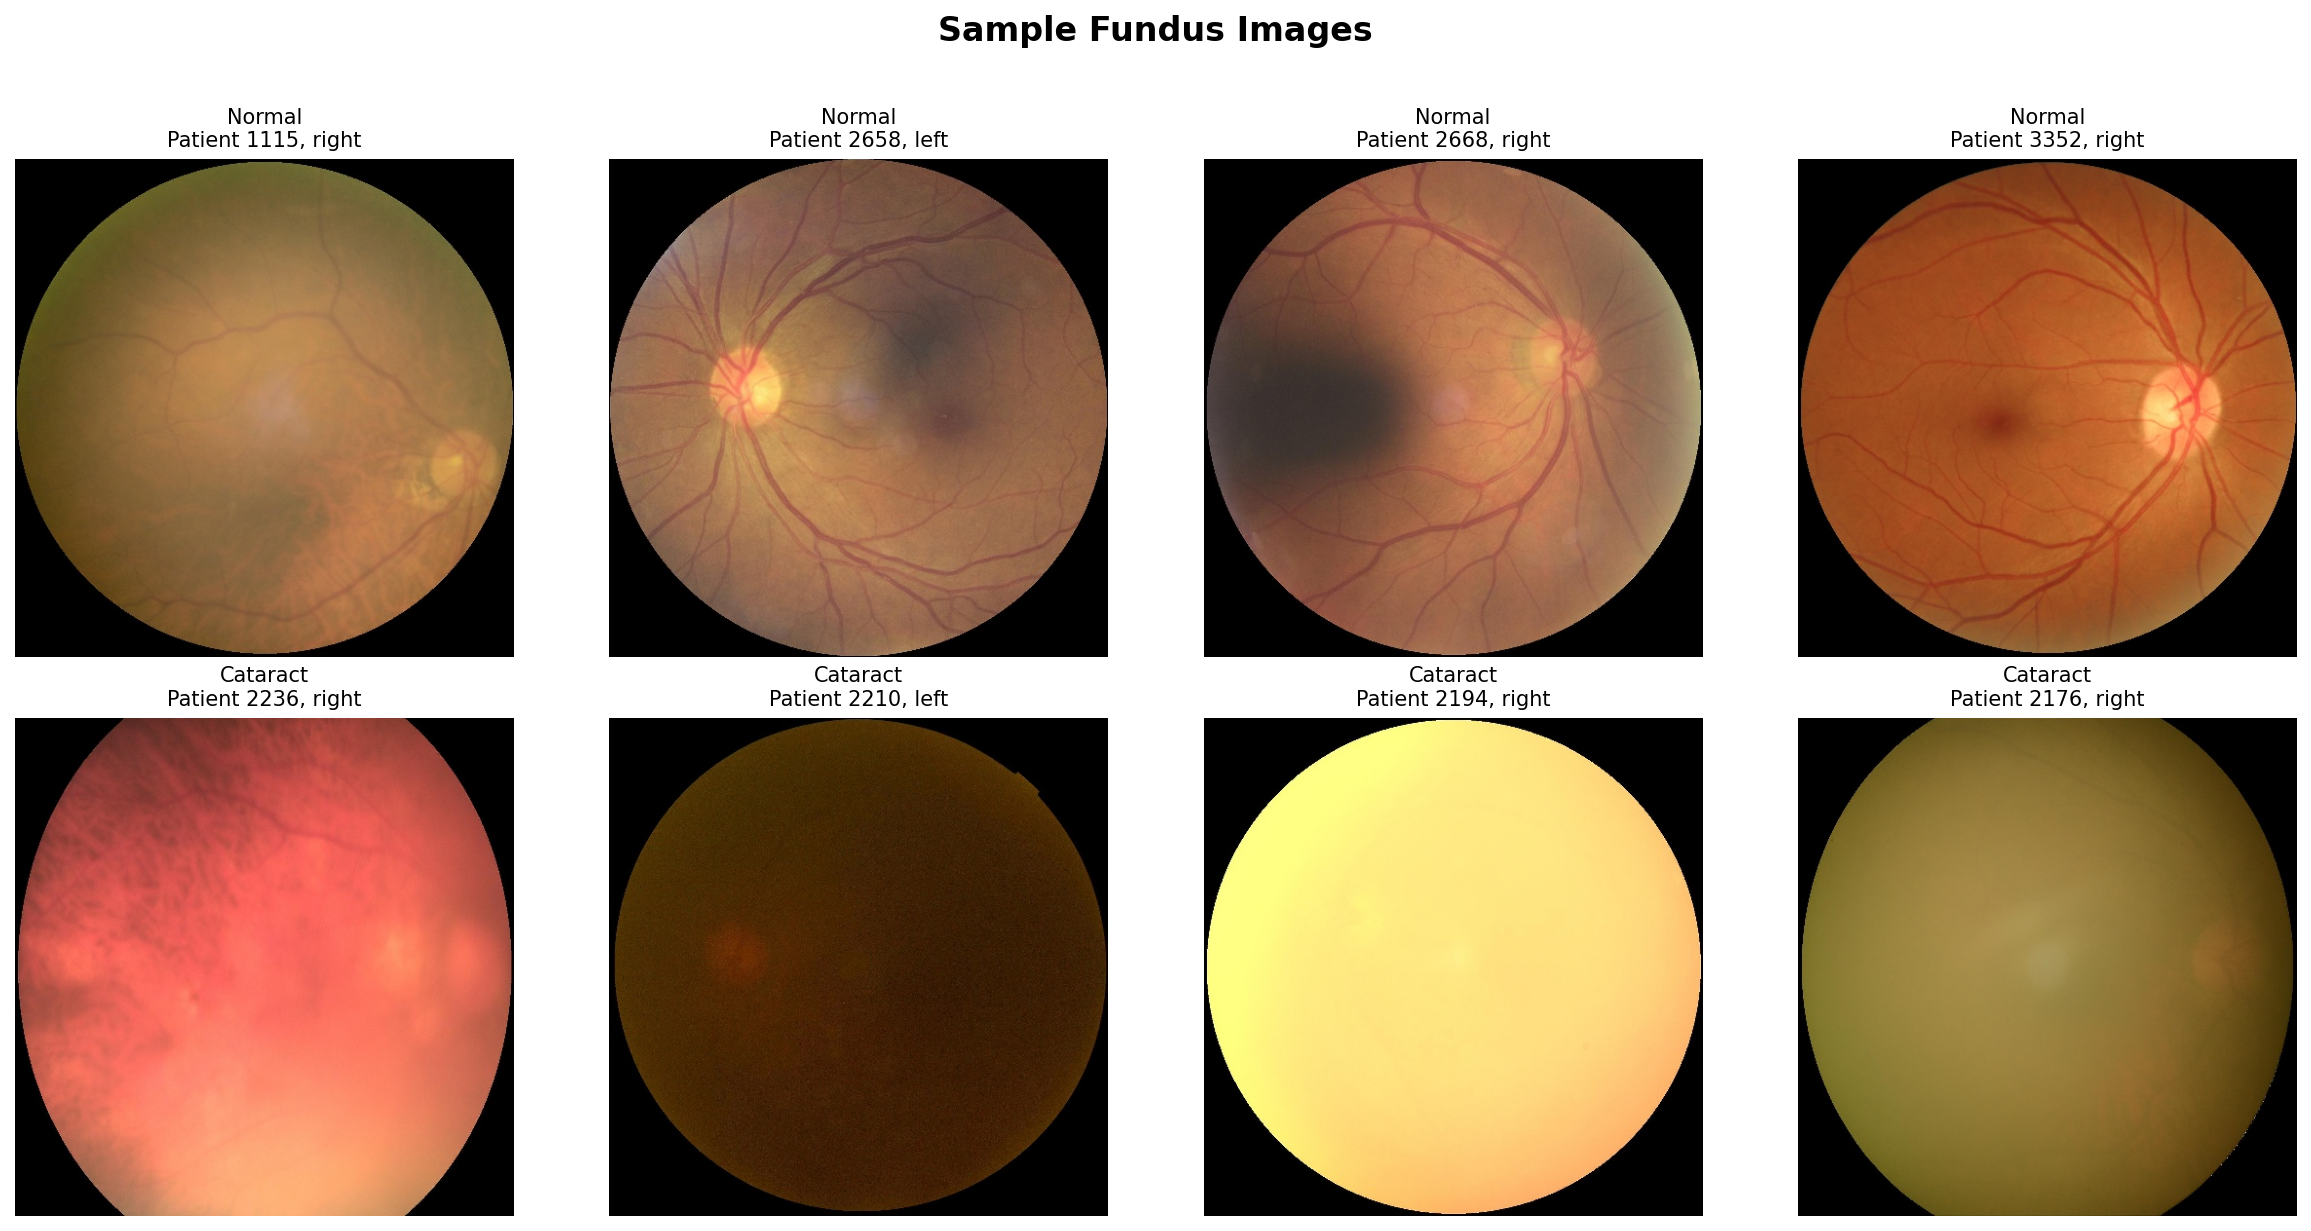
\includegraphics[width=0.95\textwidth]{figures/sample_images.png}
\caption{Sample fundus images from the normal class (top) and cataract class (bottom).}
\label{fig:samples}
\end{figure}

% ============================================================
% 6. SYSTEM ARCHITECTURE
% ============================================================
\section{System Architecture}

The system consists of two paths: an offline training/evaluation pipeline and an interactive Streamlit application. Both share the same preprocessing module to ensure consistency.

\begin{table}[H]
\centering
\begin{tabular}{@{}ll@{}}
\toprule
\textbf{Module} & \textbf{Responsibility} \\
\midrule
\texttt{src/prepare\_data.py} & Label extraction, patient-level splitting, EDA plots \\
\texttt{src/dataset.py} & PyTorch Dataset with train/eval transforms \\
\texttt{src/models.py} & ResNet50 and EfficientNet-B0 with custom head \\
\texttt{src/train.py} & AdamW training loop, early stopping, checkpoints \\
\texttt{src/evaluate.py} & Threshold selection, test metrics, comparison plots \\
\texttt{src/gradcam.py} & Grad-CAM heatmap generation \\
\texttt{app/streamlit\_app.py} & Interactive upload, prediction, Grad-CAM overlay \\
\bottomrule
\end{tabular}
\caption{System modules and their responsibilities}
\end{table}

% ============================================================
% 7. METHODOLOGY
% ============================================================
\section{Methodology}

\subsection{Preprocessing}
All images are resized to $224 \times 224$ pixels, scaled to $[0, 1]$, and normalized with ImageNet mean $(0.485, 0.456, 0.406)$ and standard deviation $(0.229, 0.224, 0.225)$. Training images receive additional augmentation: random horizontal flip (probability 0.5), rotation up to $\pm 10°$, and brightness/contrast jitter of 0.1. Validation and test images receive no augmentation.

\subsection{Model Architectures}

\subsubsection{ResNet50}
ResNet50 (He et al., 2016) uses residual connections to train very deep networks. The model has 23.5 million parameters. We load ImageNet pretrained weights, freeze all layers except \texttt{layer4} (the last convolutional block), and replace the final fully connected layer with a single-output linear layer for binary classification. This results in 15.0 million trainable parameters (63.7\%).

\subsubsection{EfficientNet-B0}
EfficientNet-B0 (Tan and Le, 2019) uses compound scaling to balance network depth, width, and resolution. The model has 4.0 million parameters. We freeze all layers except the last feature block and replace the classifier with a dropout layer (p=0.2) followed by a single-output linear layer. This results in 0.41 million trainable parameters (10.3\%).

\subsection{Training Configuration}

\begin{table}[H]
\centering
\begin{tabular}{@{}ll@{}}
\toprule
\textbf{Parameter} & \textbf{Value} \\
\midrule
Loss function & Binary Cross-Entropy with logits \\
Positive class weight & 10.6935 (ratio of normal to cataract in training set) \\
Optimizer & AdamW (lr = $10^{-4}$, weight decay = 0.01) \\
LR scheduler & ReduceLROnPlateau (patience = 2, factor = 0.5) \\
Maximum epochs & 15 \\
Early stopping & Patience = 5 (on validation ROC-AUC) \\
Batch size & 16 \\
Random seed & 42 \\
\bottomrule
\end{tabular}
\caption{Training hyperparameters}
\end{table}

\subsection{Threshold Selection}
After training, the validation set is scored with probabilities from 0.05 to 0.95 in steps of 0.01. The threshold that maximizes cataract F1 is selected and frozen. This threshold is applied once to the held-out test set. The deployed model is the one with the highest validation ROC-AUC.

\subsection{Grad-CAM (Gradient-weighted Class Activation Mapping)}
Grad-CAM (Selvaraju et al., 2017) produces visual explanations by computing the importance weights of each feature map in the final convolutional layer with respect to the class score. For feature maps $A^k$ and class score $y^c$:

\begin{equation}
\alpha_k^c = \frac{1}{Z} \sum_i \sum_j \frac{\partial y^c}{\partial A_{ij}^k}
\end{equation}

\begin{equation}
L^c_{\text{Grad-CAM}} = \text{ReLU}\left(\sum_k \alpha_k^c \cdot A^k\right)
\end{equation}

The resulting heatmap is resized to match the input image and overlaid to show which regions the model focused on. For ResNet50, the target layer is \texttt{layer4[-1]}; for EfficientNet-B0, it is \texttt{features[-1]}.

% ============================================================
% 8. RESULTS AND ANALYSIS
% ============================================================
\section{Results and Analysis}

\subsection{Training Results}

ResNet50 reached its best validation ROC-AUC (0.9953) at epoch 1 and early-stopped at epoch 6. The model's training accuracy rose from 89.6\% to 98.6\%, while validation AUC declined after epoch 1, indicating the large trainable parameter count allowed quick fitting.

EfficientNet-B0 improved validation ROC-AUC gradually through epoch 12 (0.9893) and trained for all 15 epochs. With only 0.41 million trainable parameters, training was more stable but slower to converge.

% ── FIGURE: Training Curves ──
\begin{figure}[H]
\centering
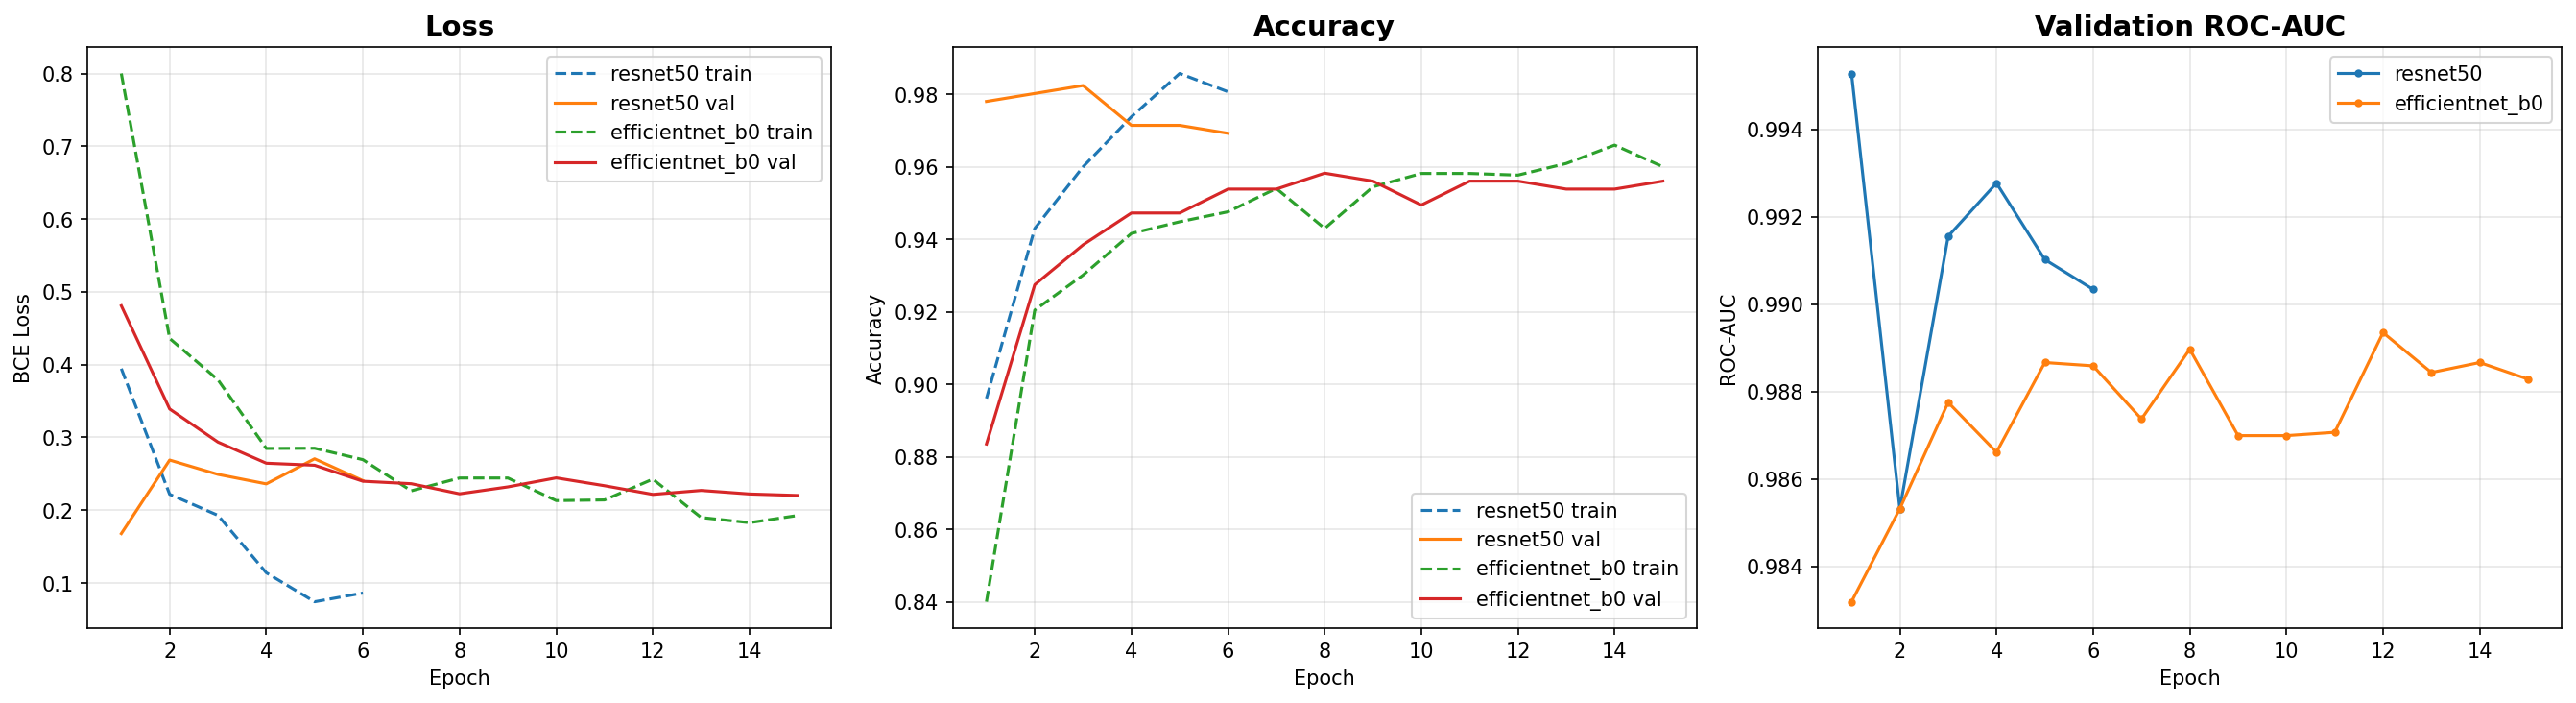
\includegraphics[width=\textwidth]{figures/training_curves.png}
\caption{Training and validation loss, accuracy, and ROC-AUC across epochs for both models.}
\label{fig:training_curves}
\end{figure}

\begin{table}[H]
\centering
\begin{tabular}{@{}lcccc@{}}
\toprule
\textbf{Model} & \textbf{Best Epoch} & \textbf{Epochs Run} & \textbf{Val ROC-AUC} & \textbf{Threshold} \\
\midrule
ResNet50 & 1 & 6 (early stop) & 0.9953 & 0.89 \\
EfficientNet-B0 & 12 & 15 & 0.9893 & 0.88 \\
\bottomrule
\end{tabular}
\caption{Training summary for both models}
\end{table}

\subsection{Test Set Performance}

The test split contains 448 images: 45 cataract and 403 normal.

\begin{table}[H]
\centering
\begin{tabular}{@{}lcc@{}}
\toprule
\textbf{Metric} & \textbf{ResNet50} & \textbf{EfficientNet-B0} \\
\midrule
Accuracy & 96.88\% & 95.31\% \\
Cataract Precision & 87.80\% & 72.22\% \\
Cataract Recall (Sensitivity) & 80.00\% & 86.67\% \\
Specificity & 98.76\% & 96.28\% \\
Cataract F1 Score & 83.72\% & 78.79\% \\
ROC-AUC & 0.9676 & 0.9848 \\
PR-AUC & 0.8943 & 0.8635 \\
\bottomrule
\end{tabular}
\caption{Test set metrics for both models}
\label{tab:results}
\end{table}

% ── FIGURE: Metrics Comparison ──
\begin{figure}[H]
\centering
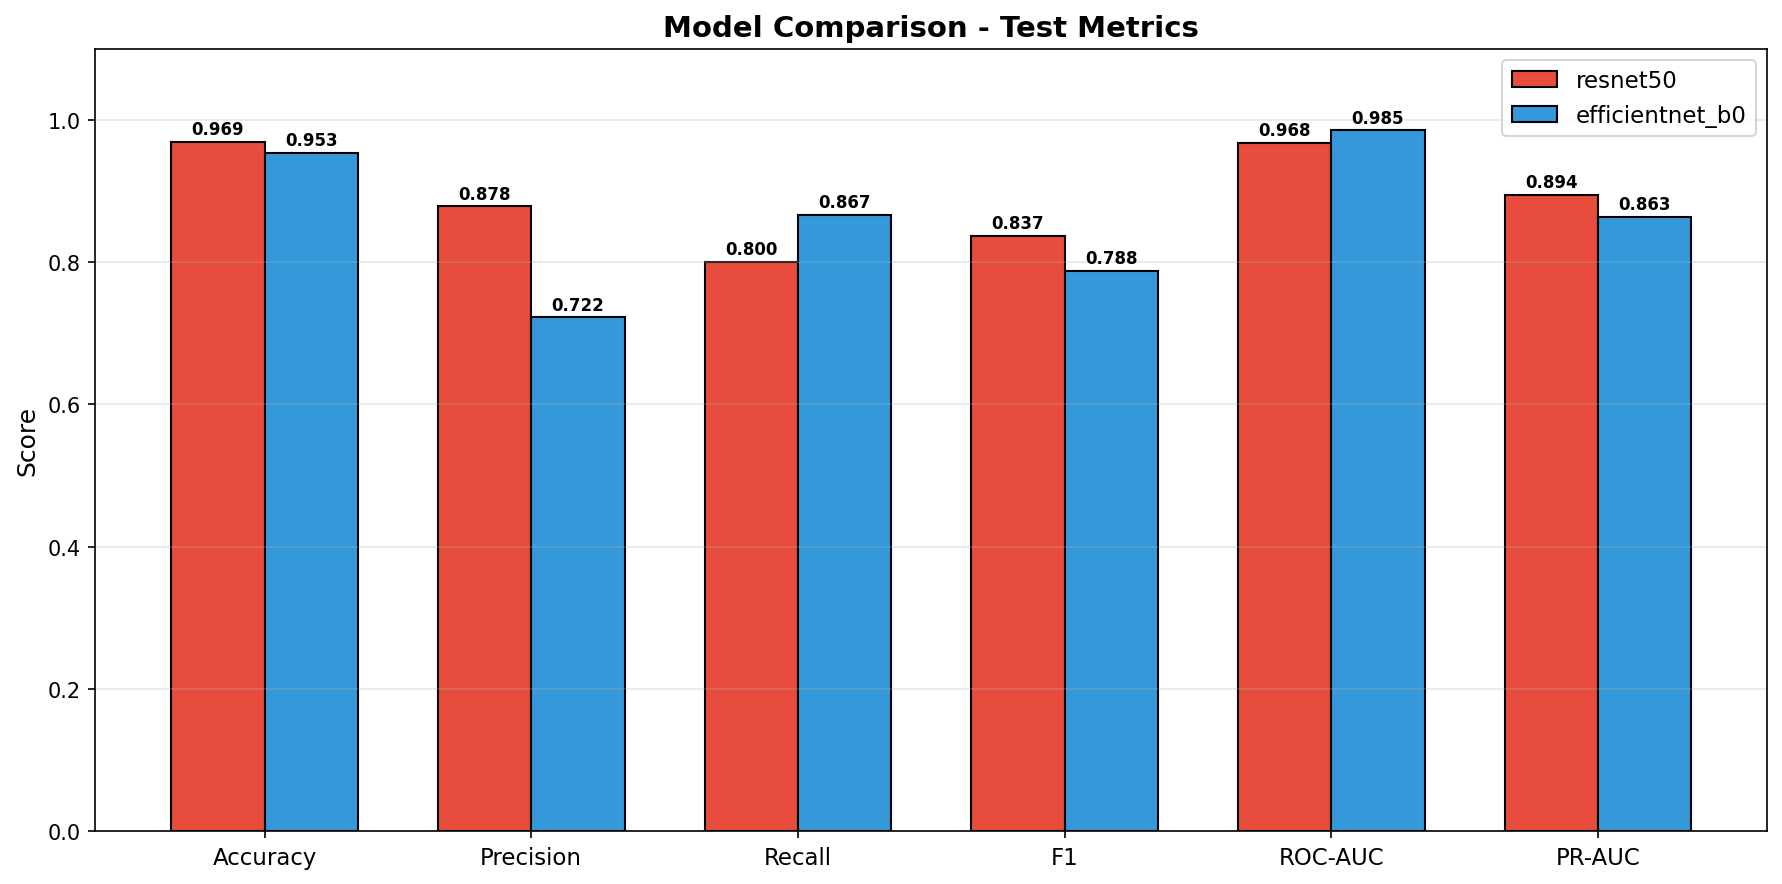
\includegraphics[width=0.9\textwidth]{figures/metrics_comparison.png}
\caption{Bar chart comparing test metrics across both models.}
\label{fig:metrics_comp}
\end{figure}

\subsection{Confusion Matrices}

\begin{figure}[H]
\centering
\begin{subfigure}{0.48\textwidth}
    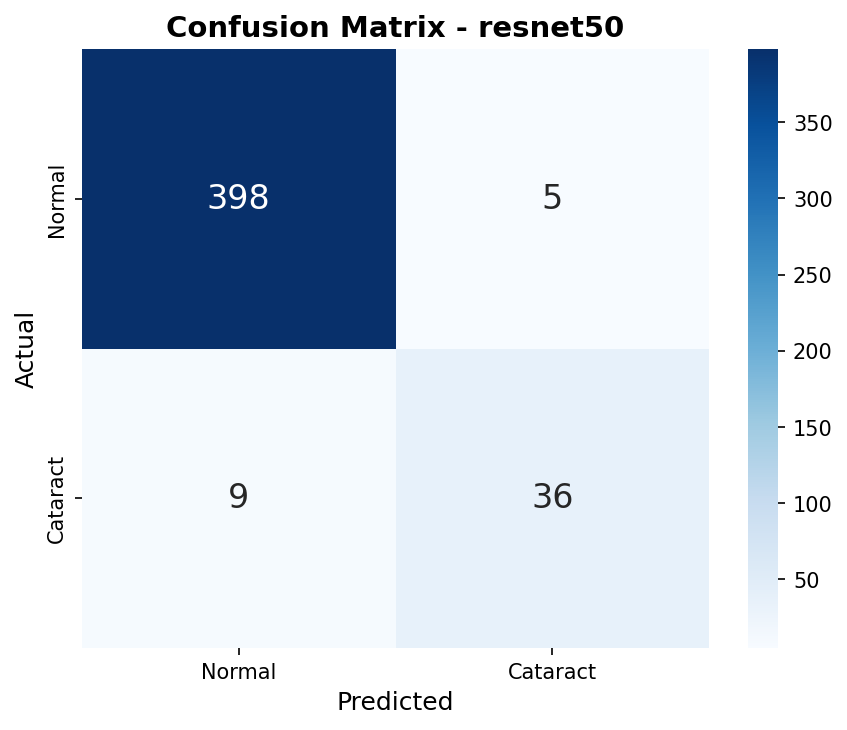
\includegraphics[width=\textwidth]{figures/confusion_matrix_resnet50.png}
    \caption{ResNet50 (threshold = 0.89)}
\end{subfigure}
\hfill
\begin{subfigure}{0.48\textwidth}
    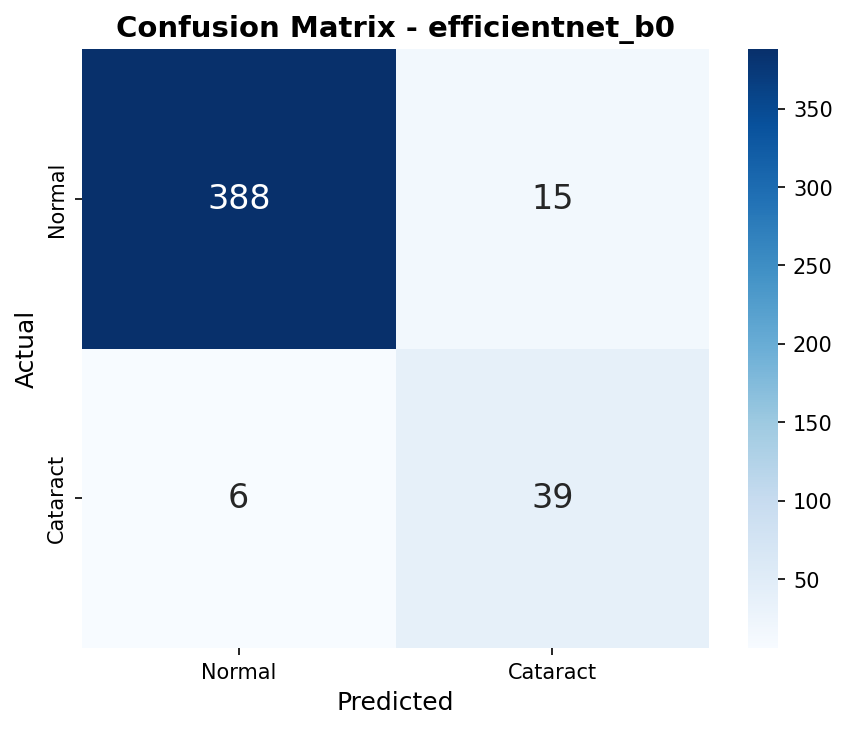
\includegraphics[width=\textwidth]{figures/confusion_matrix_efficientnet_b0.png}
    \caption{EfficientNet-B0 (threshold = 0.88)}
\end{subfigure}
\caption{Confusion matrices on the held-out test set.}
\label{fig:confusion}
\end{figure}

\begin{table}[H]
\centering
\begin{tabular}{@{}lcccc@{}}
\toprule
\textbf{Model} & \textbf{True Normal} & \textbf{False Cataract} & \textbf{Missed Cataract} & \textbf{True Cataract} \\
\midrule
ResNet50 & 398 & 5 & 9 & 36 \\
EfficientNet-B0 & 388 & 15 & 6 & 39 \\
\bottomrule
\end{tabular}
\caption{Confusion matrix values for both models}
\end{table}

\subsection{ROC and Precision-Recall Curves}

\begin{figure}[H]
\centering
\begin{subfigure}{0.48\textwidth}
    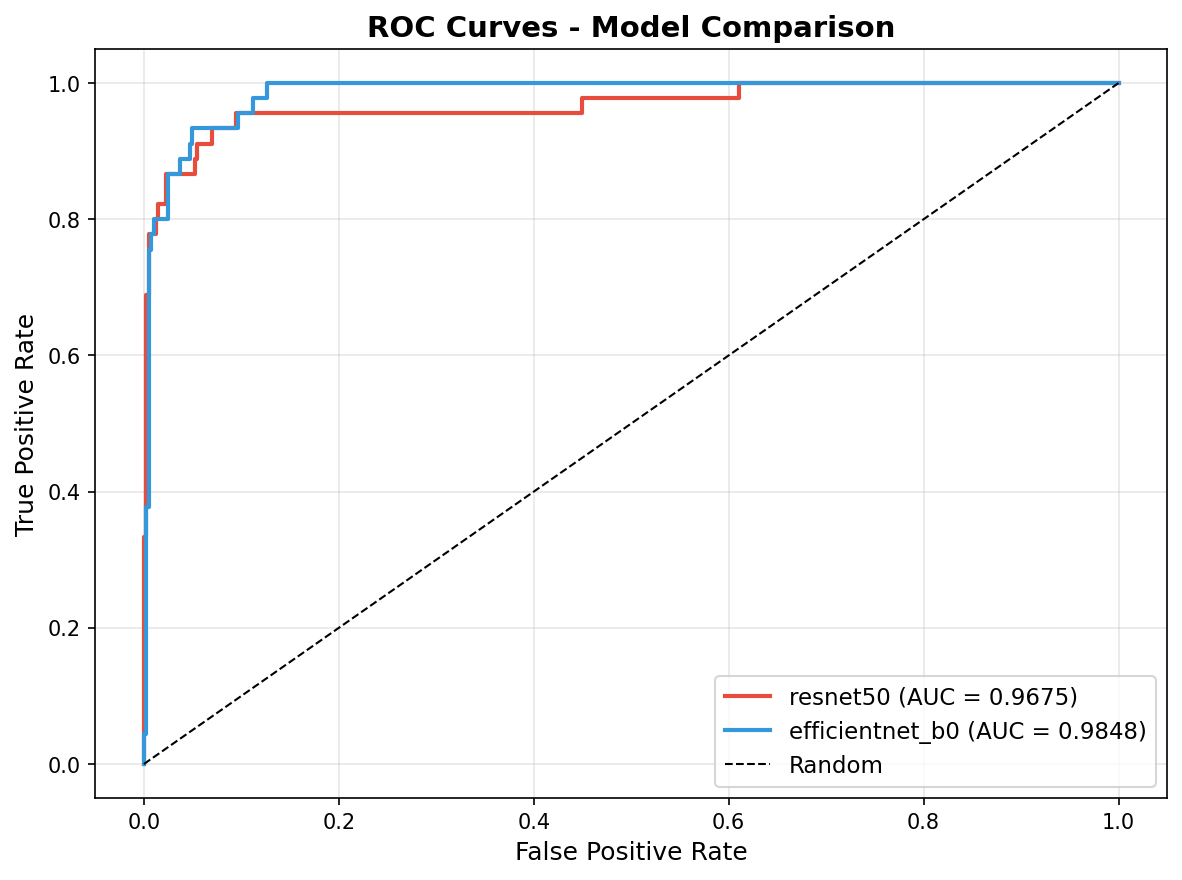
\includegraphics[width=\textwidth]{figures/roc_curves_comparison.png}
    \caption{ROC curves}
\end{subfigure}
\hfill
\begin{subfigure}{0.48\textwidth}
    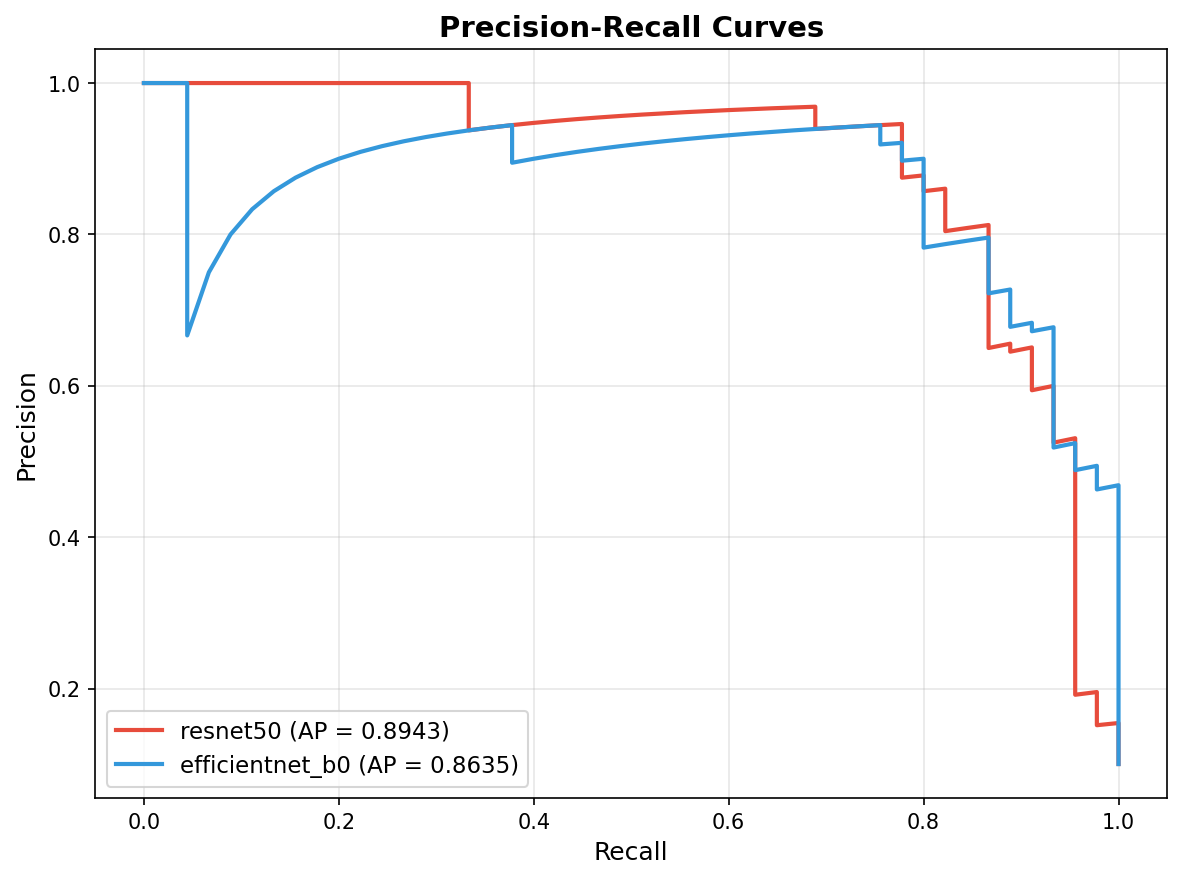
\includegraphics[width=\textwidth]{figures/pr_curves_comparison.png}
    \caption{Precision-Recall curves}
\end{subfigure}
\caption{ROC and Precision-Recall curves comparing both models on the test set.}
\label{fig:curves}
\end{figure}

\subsection{Analysis}
ResNet50 was selected as the deployed model because its validation ROC-AUC (0.9953) exceeded EfficientNet-B0's (0.9893). On the test set, ResNet50 has higher accuracy (96.88\% vs 95.31\%), higher precision (87.80\% vs 72.22\%), and higher F1 (83.72\% vs 78.79\%). EfficientNet-B0 has higher recall (86.67\% vs 80.00\%) and higher test ROC-AUC (0.9848 vs 0.9676), meaning it ranks images better overall but its frozen threshold produces more false positives.

The class imbalance (only 45 of 448 test images are cataract) means that one image changes recall by approximately 2.2 percentage points, so small differences should not be over-interpreted.

% ============================================================
% 9. GRAD-CAM EXPLANATIONS
% ============================================================
\section{Grad-CAM Explanations}

Grad-CAM heatmaps were generated for the deployed ResNet50 model. Each panel shows the original photograph, the Grad-CAM heatmap, and the overlay. The probability and threshold are printed on each panel.

\subsection{Correct Cataract Predictions}

\begin{figure}[H]
\centering
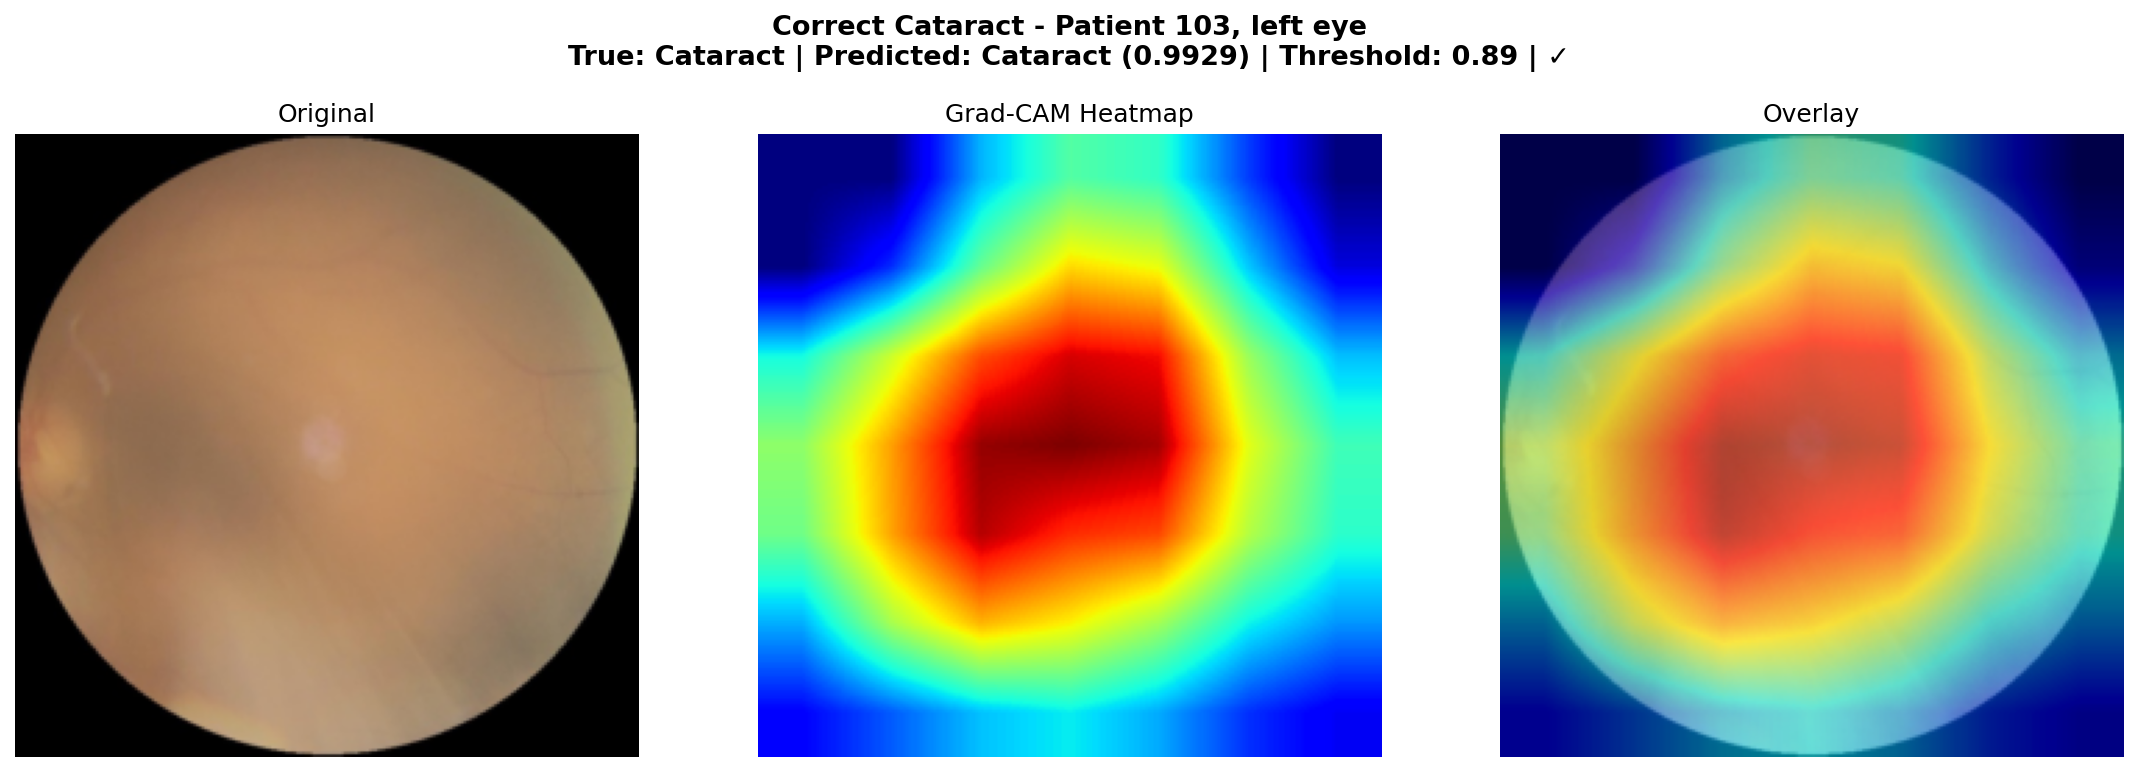
\includegraphics[width=\textwidth]{figures/gradcam_correct_cataract_1.png}
\caption{Correct cataract prediction — Example 1.}
\end{figure}

\begin{figure}[H]
\centering
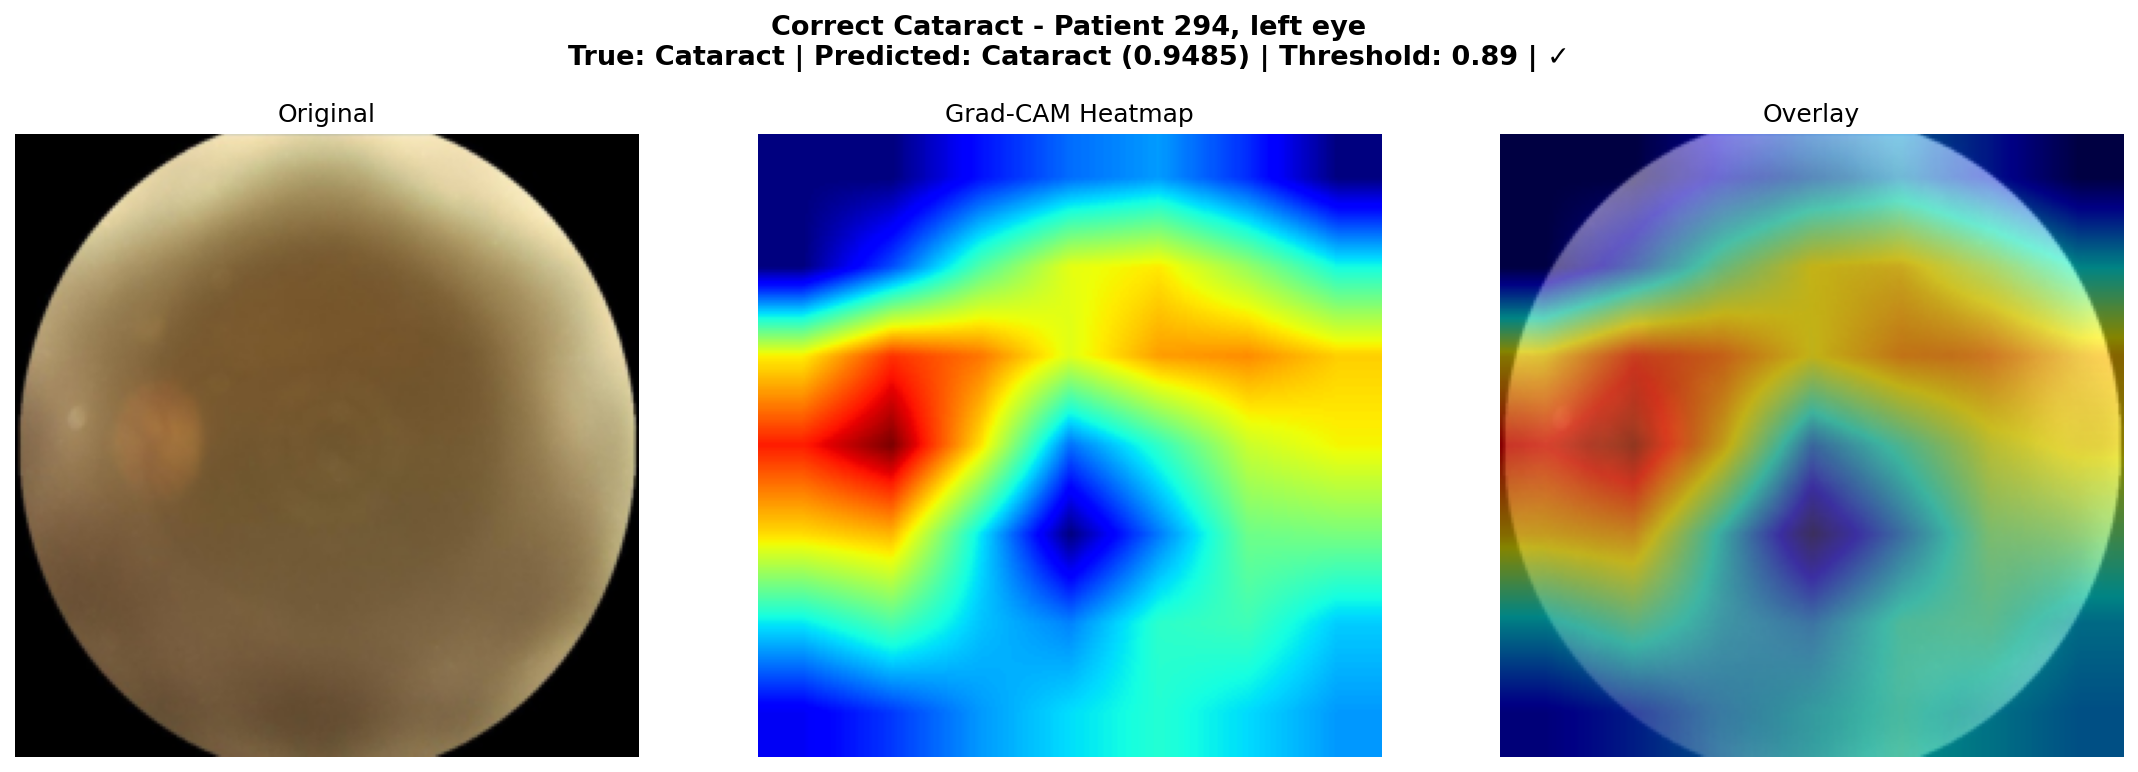
\includegraphics[width=\textwidth]{figures/gradcam_correct_cataract_2.png}
\caption{Correct cataract prediction — Example 2.}
\end{figure}

\subsection{Correct Normal Predictions}

\begin{figure}[H]
\centering
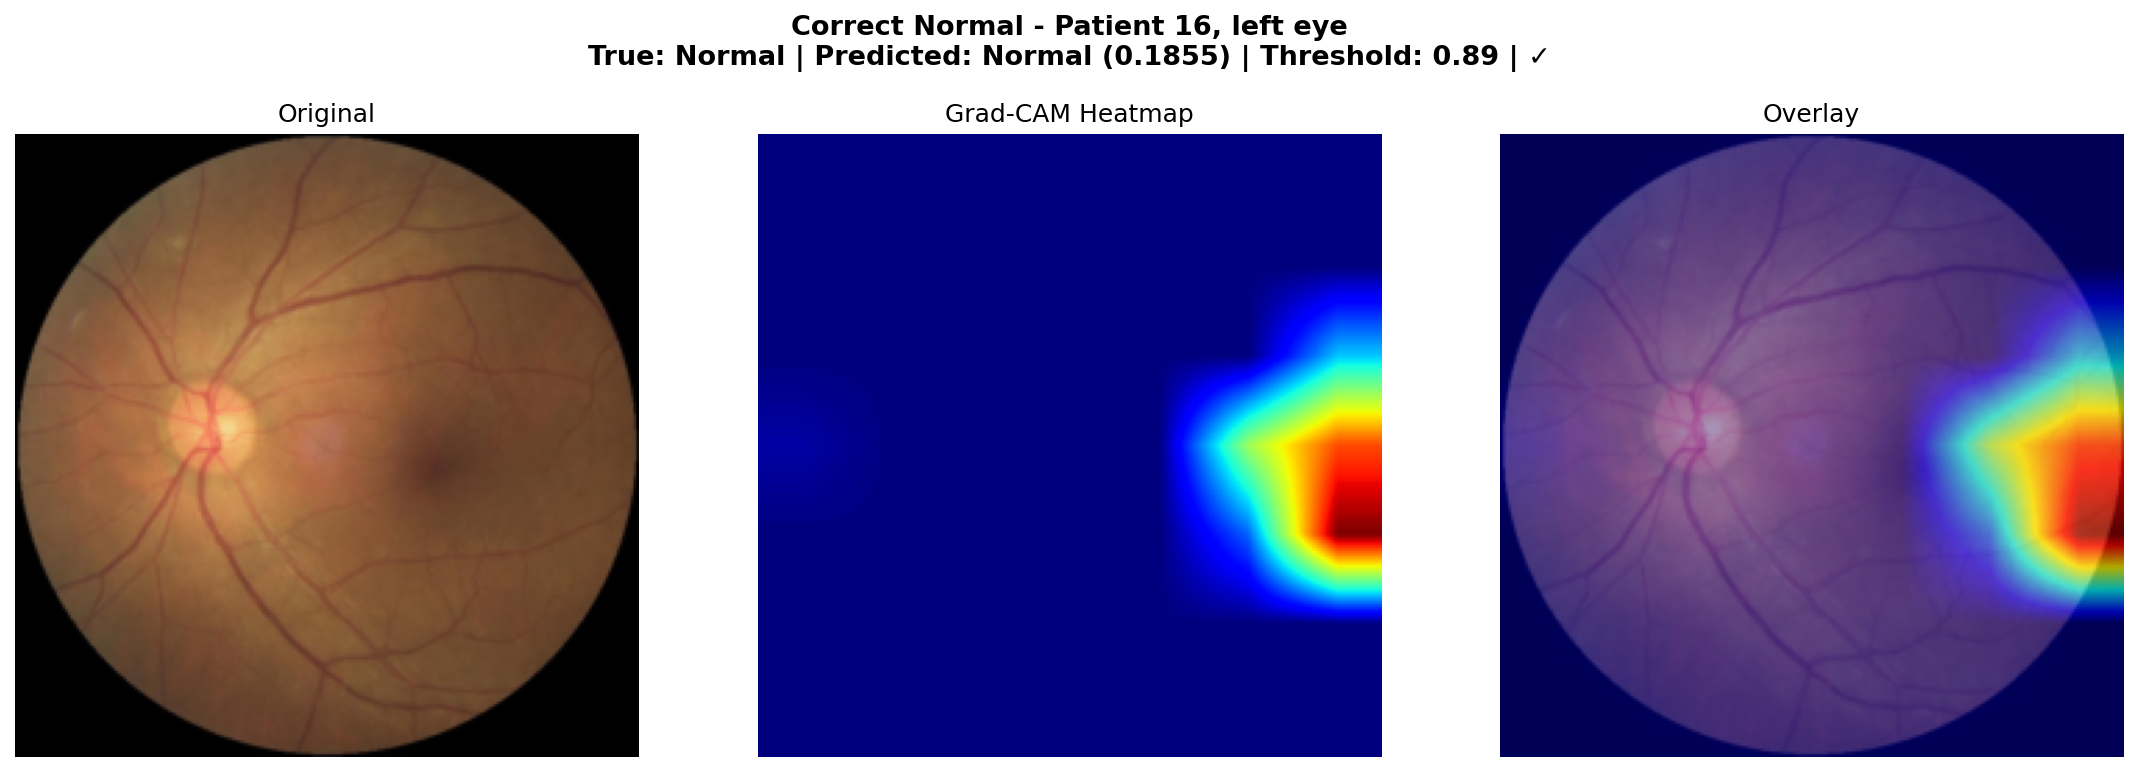
\includegraphics[width=\textwidth]{figures/gradcam_correct_normal_1.png}
\caption{Correct normal prediction — Example 1.}
\end{figure}

\begin{figure}[H]
\centering
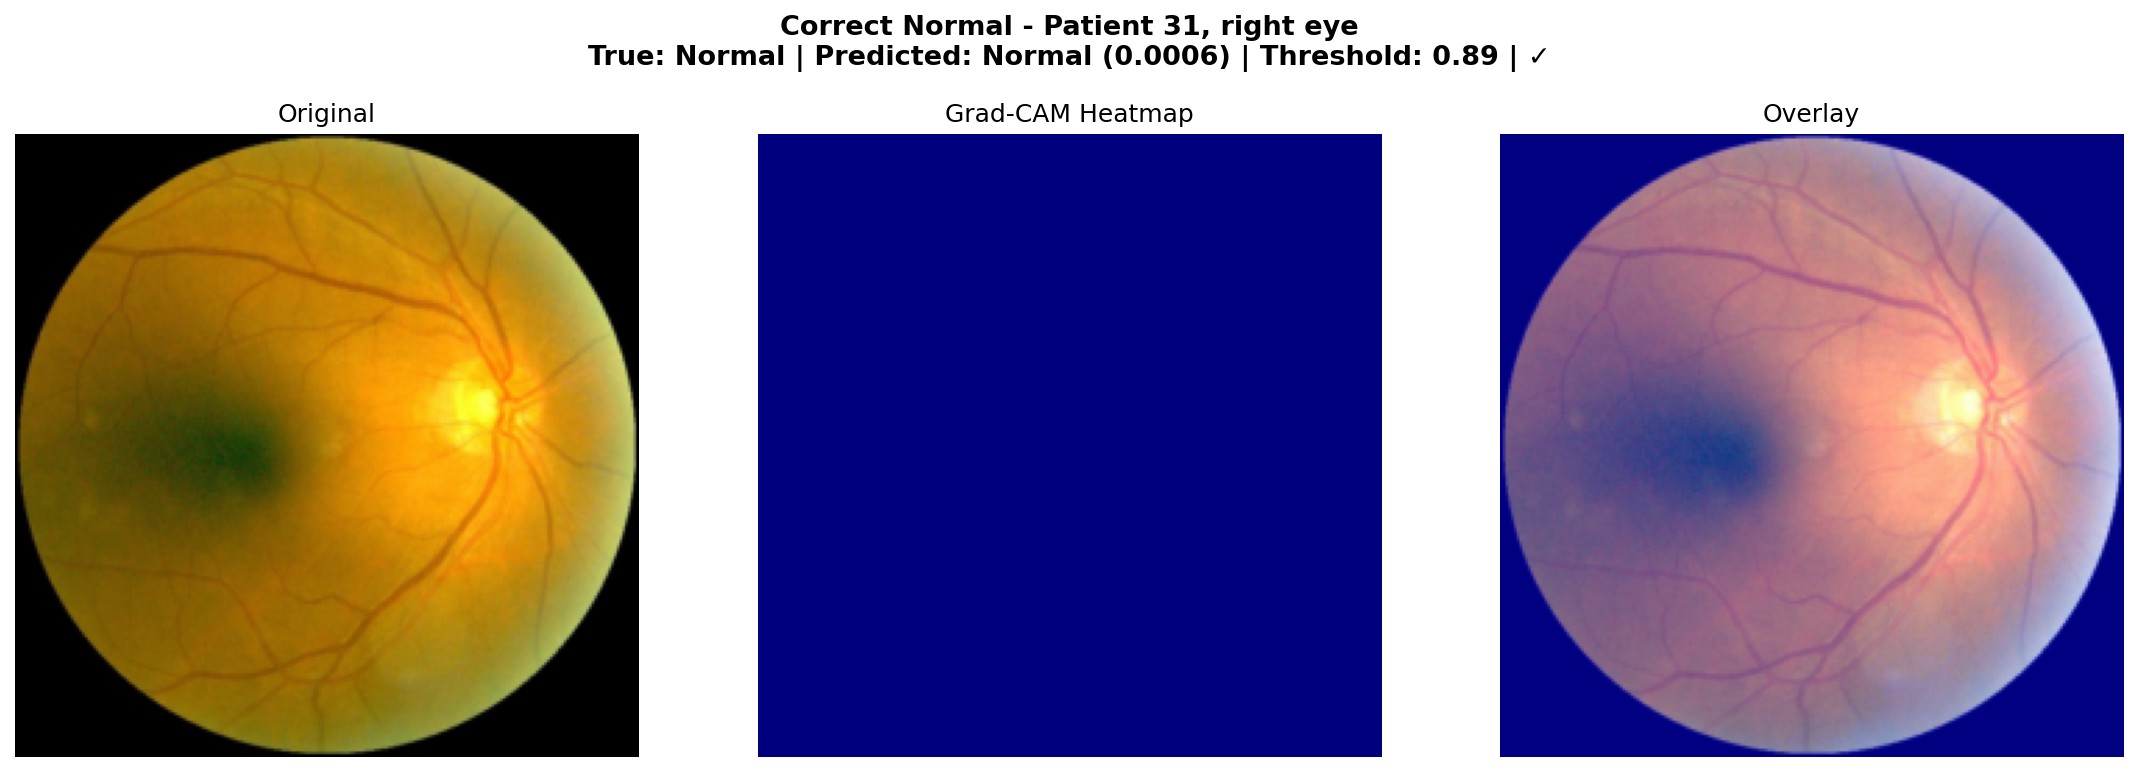
\includegraphics[width=\textwidth]{figures/gradcam_correct_normal_2.png}
\caption{Correct normal prediction — Example 2.}
\end{figure}

\subsection{Misclassified Examples}

\begin{figure}[H]
\centering
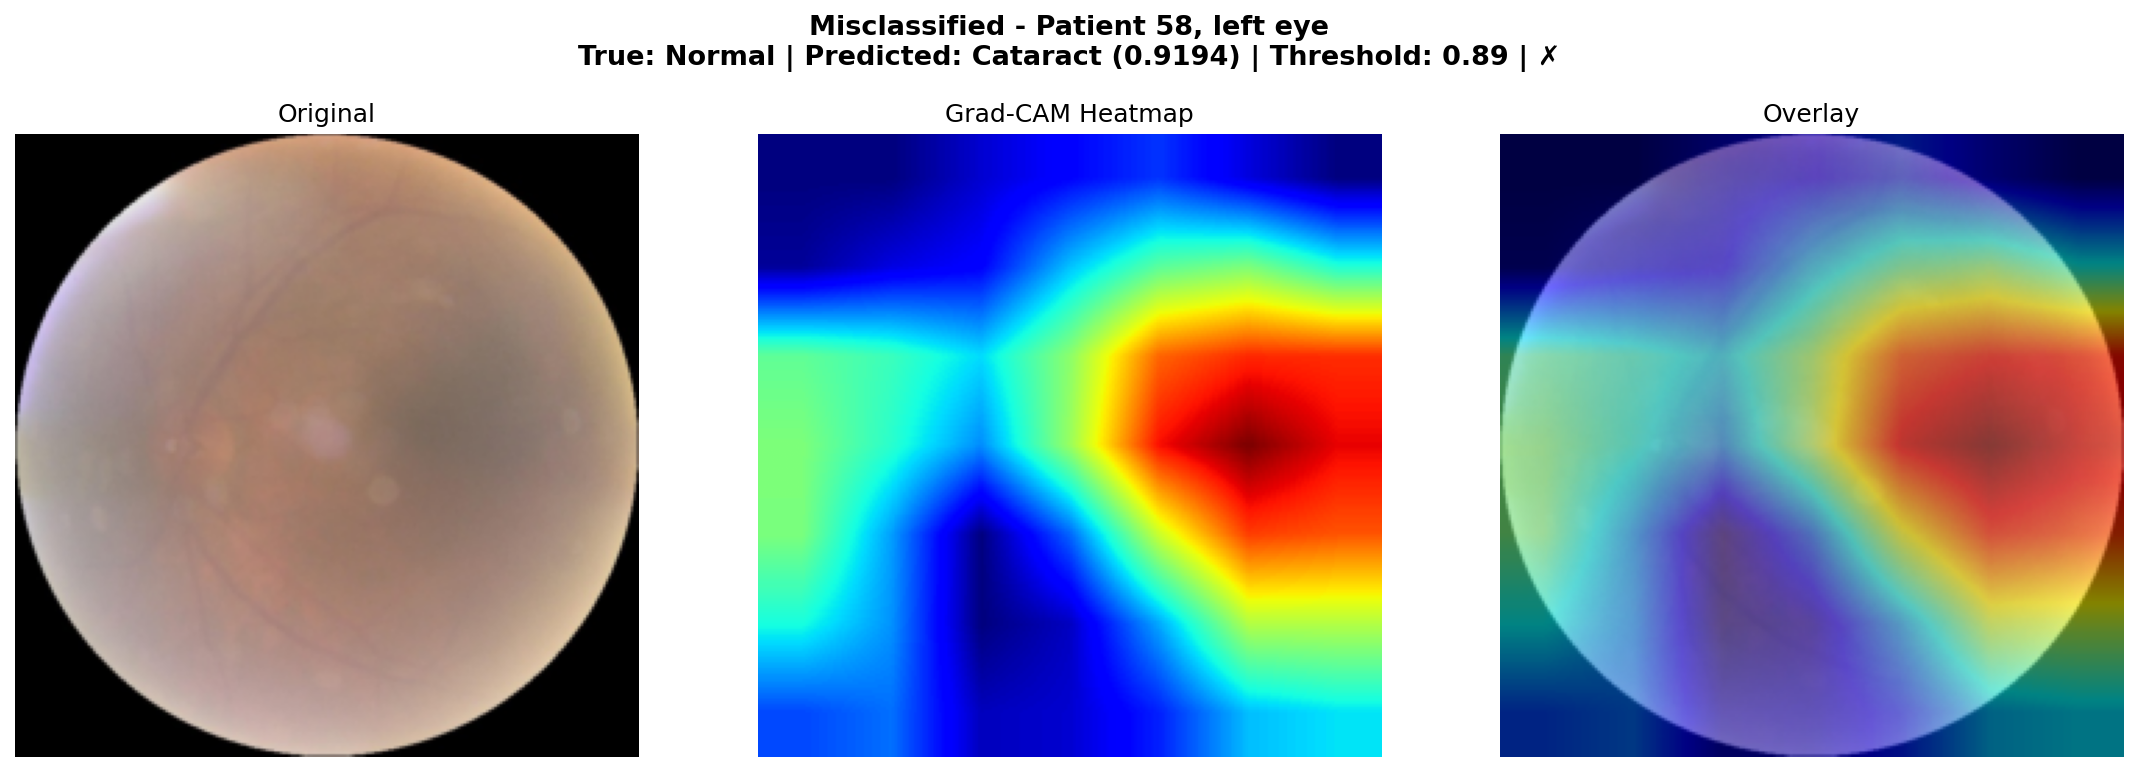
\includegraphics[width=\textwidth]{figures/gradcam_misclassified_1.png}
\caption{Misclassified example — the model's prediction was incorrect.}
\end{figure}

\begin{figure}[H]
\centering
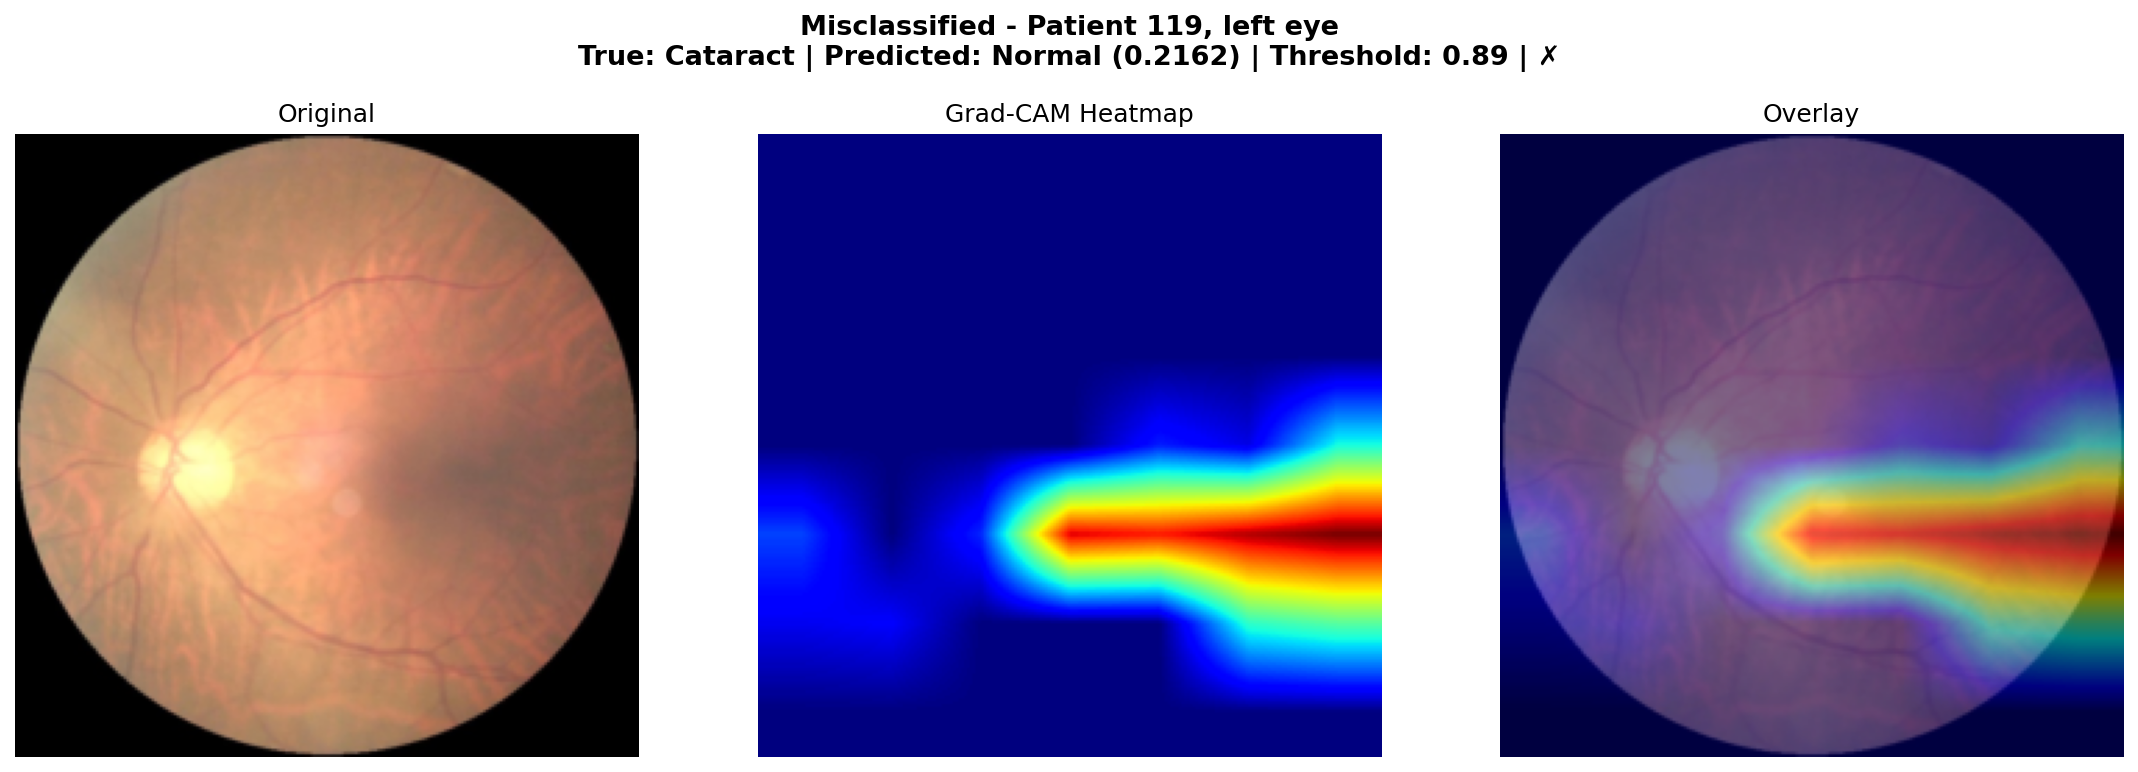
\includegraphics[width=\textwidth]{figures/gradcam_misclassified_2.png}
\caption{Misclassified example — the model's prediction was incorrect.}
\end{figure}

\subsection{Observations}
The Grad-CAM heatmaps show that for correctly classified cataract images, the model focuses on the central fundus region where cataract-induced haze and contrast changes are most visible. For normal images, the model's attention is more distributed or focused on the optic disc region. These maps explain the model's score but do not outline the lens itself, since the fundus camera photographs the retina through the lens.

% ============================================================
% 10. STREAMLIT APPLICATION
% ============================================================
\section{Streamlit Web Application}

A Streamlit-based web application provides an interactive demo. Users can upload a retinal fundus image, and the application displays:
\begin{itemize}
    \item The predicted class (Cataract or Normal)
    \item The cataract probability score
    \item The frozen decision threshold
    \item A Grad-CAM overlay showing the model's focus regions
\end{itemize}

The application is launched with the command:
\begin{lstlisting}
streamlit run app/streamlit_app.py
\end{lstlisting}

% ── SCREENSHOT NOTE ──
% Take a screenshot of the running Streamlit app and save as:
% report/figures/streamlit_app.png
% Then uncomment the figure below:

% \begin{figure}[H]
% \centering
% \includegraphics[width=0.9\textwidth]{figures/streamlit_app.png}
% \caption{Streamlit web application showing cataract prediction with Grad-CAM.}
% \label{fig:streamlit}
% \end{figure}

% ============================================================
% 11. CONCLUSION
% ============================================================
\section{Conclusion}

This project demonstrates that transfer learning with pretrained ImageNet models can effectively classify retinal fundus images as cataract or normal using the ODIR-5K dataset. The key findings are:

\begin{enumerate}
    \item \textbf{ResNet50} achieved the best validation ROC-AUC (0.9953) and was selected as the deployed model, with test accuracy of 96.88\%, precision of 87.80\%, and F1 score of 83.72\%.
    \item \textbf{EfficientNet-B0} achieved higher test recall (86.67\%) and test ROC-AUC (0.9848) with only 4 million parameters, demonstrating efficiency.
    \item \textbf{Grad-CAM} heatmaps confirm that the model focuses on clinically relevant regions of the fundus image, increasing interpretability and trust.
    \item \textbf{Patient-level splitting} prevents data leakage between training and testing.
    \item \textbf{Weighted loss} effectively handles the significant class imbalance (8.5\% cataract).
\end{enumerate}

The system is a research prototype and not a clinical diagnostic tool. The positive test set has only 45 images, mixed diseases were removed before training, and there is no external validation dataset.

\subsection{Future Scope}
\begin{itemize}
    \item \textbf{Multi-class classification:} Extend to detect multiple eye diseases (glaucoma, diabetic retinopathy, AMD) simultaneously.
    \item \textbf{Cataract grading:} Instead of binary classification, grade cataract severity (mild, moderate, severe).
    \item \textbf{External validation:} Test on datasets from different cameras and populations.
    \item \textbf{Larger models:} Experiment with Vision Transformers (ViT) and larger EfficientNet variants.
    \item \textbf{LIME explanations:} Add LIME-based superpixel explanations alongside Grad-CAM.
    \item \textbf{Mobile deployment:} Convert the model to ONNX or TFLite for mobile screening applications.
\end{itemize}

% ============================================================
% REFERENCES
% ============================================================
\section*{References}
\addcontentsline{toc}{section}{References}

\begin{thebibliography}{99}

\bibitem{selvaraju2017}
R. R. Selvaraju, M. Cogswell, A. Das, R. Vedantam, D. Parikh, and D. Batra, ``Grad-CAM: Visual explanations from deep networks via gradient-based localization,'' in \textit{Proc. IEEE Int. Conf. Comput. Vis. (ICCV)}, 2017.

\bibitem{he2016}
K. He, X. Zhang, S. Ren, and J. Sun, ``Deep residual learning for image recognition,'' in \textit{Proc. IEEE Conf. Comput. Vis. Pattern Recognit. (CVPR)}, 2016, pp. 770--778.

\bibitem{tan2019}
M. Tan and Q. Le, ``EfficientNet: Rethinking model scaling for convolutional neural networks,'' in \textit{Proc. 36th Int. Conf. Mach. Learn. (ICML)}, PMLR vol. 97, 2019, pp. 6105--6114.

\bibitem{li2021}
N. Li, T. Li, C. Hu, K. Wang, and H. Kang, ``A benchmark of ocular disease intelligent recognition: One shot for multi-disease detection,'' \textit{arXiv:2102.07978}, 2021.

\bibitem{raghu2019}
M. Raghu, C. Zhang, J. Kleinberg, and S. Bengio, ``Transfusion: Understanding transfer learning for medical imaging,'' in \textit{Adv. Neural Inf. Process. Syst. (NeurIPS)}, vol. 32, 2019, pp. 3347--3357.

\bibitem{yang2016}
M. Yang, J.-J. Yang, Q. Zhang, Y. Niu, and J. Li, ``Classification of retinal image for automatic cataract detection,'' in \textit{IEEE Int. Conf. e-Health Networking, Applications and Services (Healthcom)}, 2016.

\bibitem{ali2022}
H. H. Ali, A. Y. Al-Sultan, and E. Hamood, ``Classifying three stages of cataract disease using CNN,'' \textit{J. Univ. Babylon Pure Appl. Sci.}, vol. 30, no. 3, pp. 150--167, 2022.

\bibitem{loshchilov2019}
I. Loshchilov and F. Hutter, ``Decoupled weight decay regularization,'' in \textit{Proc. Int. Conf. Learn. Represent. (ICLR)}, 2019.

\end{thebibliography}

\end{document}

